\documentclass[12pt]{article}

% Core math
\usepackage{amsmath, amssymb, amsthm}
\usepackage{mathtools}
\usepackage{stmaryrd}

% Tables
\usepackage{tabularx}
\usepackage{booktabs}
\usepackage{array}

% Diagrams
\usepackage{tikz-cd}
\usepackage{tikz}
\usetikzlibrary{positioning, arrows.meta, calc, decorations.markings}

% References (load order: hyperref before cleveref)
\usepackage[hidelinks]{hyperref}
\usepackage{cleveref}
\usepackage{xurl}

% Graphics
\usepackage{graphicx}

% Code listings
\usepackage{listings}
\usepackage{xcolor}

% Page layout
\usepackage[margin=1in]{geometry}

% Sidebar (use modern shipout/background hook)
% (no everypage required; LaTeX provides AddToHook)

% Theorem environments
\newtheorem{theorem}{Theorem}[section]
\newtheorem{proposition}[theorem]{Proposition}
\newtheorem{lemma}[theorem]{Lemma}
\newtheorem{corollary}[theorem]{Corollary}
\theoremstyle{definition}
\newtheorem{definition}[theorem]{Definition}
\newtheorem{example}[theorem]{Example}
\newtheorem{principle}[theorem]{Principle}
\theoremstyle{remark}
\newtheorem{remark}[theorem]{Remark}

% Listings styling for Haskell
\lstdefinelanguage{Haskell}{
  morekeywords={data, type, class, instance, where, let, in, do, case, of,
    if, then, else, module, import, newtype, deriving, family, forall},
  sensitive=true,
  morecomment=[l]{--},
  morestring=[b]"
}
\lstset{
  basicstyle=\ttfamily\small,
  keywordstyle=\color{blue!70!black}\bfseries,
  commentstyle=\color{green!50!black}\itshape,
  stringstyle=\color{red!70!black},
  showstringspaces=false,
  breaklines=true,
  frame=single,
  framesep=4pt,
  rulecolor=\color{gray!50},
  language=Haskell
}

% GrokRxiv sidebar (first page)
\definecolor{grokgray}{RGB}{110,110,110}
\AddToHook{shipout/background}{%
  \ifnum\value{page}=1
    \begin{tikzpicture}[remember picture, overlay]
      \node[
        rotate=90,
        anchor=south,
        font=\Large\sffamily\bfseries\color{grokgray},
        inner sep=0pt
      ] at ([xshift=38pt, yshift=0.52\paperheight]current page.south west)
      {GrokRxiv:2026.05.univalent-correspondence-synthesis\quad
       [\,math.CT/math.LO\,]\quad
       03 May 2026};
    \end{tikzpicture}
  \fi
}

% Macros
\newcommand{\N}{\mathbb{N}}
\newcommand{\Z}{\mathbb{Z}}
\newcommand{\Q}{\mathbb{Q}}
\newcommand{\R}{\mathbb{R}}
\newcommand{\C}{\mathbb{C}}
\newcommand{\Set}{\mathbf{Set}}
\newcommand{\Cat}{\mathbf{Cat}}
\newcommand{\Grpd}{\mathbf{Gpd}}
\newcommand{\PtEndo}{\mathbf{PtEndo}}
\newcommand{\Type}{\mathsf{Type}}
\newcommand{\U}{\mathcal{U}}
\newcommand{\op}{^{\mathrm{op}}}
\newcommand{\id}{\mathrm{id}}
\newcommand{\Hom}{\mathrm{Hom}}
\newcommand{\Nat}{\mathrm{Nat}}
\newcommand{\zero}{\mathsf{zero}}
\newcommand{\suc}{\mathsf{succ}}
\newcommand{\Id}{\mathsf{Id}}
\newcommand{\refl}{\mathsf{refl}}
\newcommand{\transport}{\mathsf{transport}}
\newcommand{\ua}{\mathsf{ua}}
\newcommand{\idtoeqv}{\mathsf{idtoeqv}}
\newcommand{\eqv}{\simeq}
\newcommand{\iso}{\cong}
\newcommand{\isContr}{\mathsf{isContr}}
\newcommand{\isProp}{\mathsf{isProp}}
\newcommand{\isSet}{\mathsf{isSet}}
\newcommand{\NNO}{\mathrm{NNO}}

\title{The Univalent Correspondence: \\
How Six Perspectives on Number Become One \\
\large Synthesis of the Univalent Correspondence Series}

\author{YonedaAI Research \\
\textit{Univalent Correspondence Project} \\
\textit{Synthesis paper for the six topical papers (I--VI)} \\
\texttt{research@yonedaai.com}}

\date{3 May 2026}

\begin{document}
\maketitle

\begin{abstract}
This is the synthesis paper for the six-part series \emph{The Univalent
Correspondence}. Each topical paper takes one perspective on the question
``what is the natural number $58$?'' and develops it to maturity: Paper~I
treats $58$ naively as a symbol or quantity; Paper~II encodes it
set-theoretically as a von Neumann ordinal; Paper~III characterizes it by a
universal property as the $58$th iterate of $\suc$ in any initial successor
structure; Paper~IV identifies it with its representable functor
$\Hom(-, 58)$; Paper~V realises it as a canonical term of an inductive type
$\N$ in Homotopy Type Theory, identified up to path equivalence; Paper~VI
reads it structurally, as an invariant under all structure-preserving
morphisms between models of arithmetic. We argue that under Voevodsky's
univalence axiom, the four perspectives of Papers~III through~VI are not
analogous but \emph{literally identical}: an initial successor structure, a
representing presheaf, a contractible $\Sigma$-type of NNO structures, and a
structural invariant of arithmetic models are four faces of one
$\infty$-groupoid. We name this identification the \emph{univalent
correspondence}, building on the four-way computational tetrad of Curry,
Howard, Lambek, and Voevodsky (extending Wadler's
propositions-as-types-as-spaces and Harper's computational trinity). After
reviewing each level, motivating the canonical six-row table, and making the
unifying $\infty$-groupoid framework precise, we prove transit theorems
showing that each level transcends its predecessor: the set-theoretic level
resolves the naive symbol/object confusion but introduces
encoding-relativity (Benacerraf's identification problem); the universal
property resolves encoding by going relational; Yoneda makes ``relational
profile'' mathematically precise as a representable functor; HoTT makes
Yoneda's ``iff'' into a literal identity in the universe via univalence;
and the categorical/structural perspective is the philosophical commitment
that \emph{all of this} is what mathematical objects are. We close with a
research outlook on ContextFS / typed memory as a structural-identity
primitive, transcendentals $\pi$ and $e$ in HoTT via Cauchy reals as a
higher inductive--inductive type, directed HoTT and synthetic
$\infty$-category theory, and the principal open problem: a synthetic
foundation for analytic number theory.
\end{abstract}

\tableofcontents
\bigskip

\section{Introduction}
\label{sec:intro}

\subsection{The question and the six perspectives}

The Univalent Correspondence series asks one question --- \emph{what is the
natural number $58$?} --- and answers it six different ways. The six papers
of the series each occupy one row of \cref{tab:six-rows}, the central
organizing artifact of the project. The synthesis paper before you argues
that the rightmost four rows describe the \emph{same} mathematical object,
identified up to equivalence by Voevodsky's univalence axiom.

\begin{table}[ht]
\centering
\begin{tabularx}{\textwidth}{l X}
\toprule
\textbf{Level (Paper)} & \textbf{What $58$ is at this level} \\
\midrule
Naive (I) & A symbol on the page; a quantity counted by a finger or scratch. \\
Set-theoretic (II) & The von Neumann ordinal $\{0, 1, \ldots, 57\}$; equivalently, any iso-class of ZFC encodings of the same Peano structure. \\
Universal property (III) & The $58$-th iterate $\suc^{58}(\zero)$ in \emph{any} initial successor structure $(N, 0, \suc)$ in any category with terminal object. \\
Yoneda (IV) & The representable functor $\Hom(-, 58)$ on the appropriate category; equivalently, the entire system of probes that land on $58$. \\
HoTT (V) & A canonical term in the inductive type $\N$, identified up to path equivalence (and hence, by univalence, identified across NNO presentations). \\
Categorical / structural (VI) & A semantic invariant, in the sense of Awodey, Resnik, and Shapiro, under all structure-preserving morphisms between models of arithmetic. \\
\bottomrule
\end{tabularx}
\caption{The six perspectives on the natural number $58$. Rows~III--VI
become literally identical under the univalence axiom (\cref{sec:transit}).}
\label{tab:six-rows}
\end{table}

The series is not a survey. Each topical paper is a self-contained
mathematical development with its own theorems, proofs, and Haskell
artifacts. Paper~I~\cite{paper-i} is historical and philosophical, anchoring
the discussion in numerals and counting; Paper~II~\cite{paper-ii}
axiomatizes ZFC, develops the von Neumann hierarchy, and proves Benacerraf's
identification problem in formal terms; Paper~III~\cite{paper-iii}
introduces the natural numbers object, derives primitive recursion from its
universal property, and shows the equivalence with second-order Peano
arithmetic; Paper~IV~\cite{paper-iv} proves the Yoneda lemma in covariant
and contravariant forms, with applications to numbers, groups, schemes, and
the $\infty$-categorical generalization; Paper~V~\cite{paper-v} is a
self-contained development of HoTT including identity types, path
induction, the univalence axiom, higher inductive types, and the cubical
realisation; Paper~VI~\cite{paper-vi} surveys mathematical structuralism,
proves an isomorphism-invariance theorem for first-order properties, and
relates categorification to decategorification.

The synthesis paper before you assumes the existence and content of these
six topical papers and combines them. We do not re-prove their main
theorems; we cite them. What we do prove are the \emph{transit theorems}
between levels, and we collect them into a single mathematical statement of
the univalent correspondence (\cref{sec:transit,sec:correspondence}).

\subsection{The thesis}

The thesis of this paper, and of the series as a whole, has two layers.

\begin{principle}[Univalent Correspondence, weak form]
\label{prin:weak}
For the natural numbers, and more generally for any mathematical
structure presentable by an essentially algebraic theory, the four
perspectives \emph{universal property} (Paper~III), \emph{Yoneda}
(Paper~IV), \emph{HoTT term up to path equivalence} (Paper~V), and
\emph{structural invariant} (Paper~VI) yield equivalent characterisations.
\end{principle}

\begin{principle}[Univalent Correspondence, strong form]
\label{prin:strong}
Under the univalence axiom, the equivalences of \cref{prin:weak} are
internalised as identities in a universe $\U$. The four characterisations
do not merely yield isomorphic answers; they are paths in the same
$\infty$-groupoid, and the natural number $58$ is a single point in that
$\infty$-groupoid, viewed through four windows.
\end{principle}

The strong form is the content of \cref{thm:identity-of-perspectives}
below. The weak form is established meta-theoretically by the work of
Lawvere~\cite{Lawvere1964}, Lambek~\cite{Lambek1972}, Wadler~\cite{Wadler2015},
Awodey~\cite{Awodey2014}, and the HoTT Book~\cite{HoTTBook}. The strong
form requires univalence and the structure identity principle (SIP); see
\cref{sec:transit-vi}.

\subsection{Why a sixth row?}

A natural question: if the universal property already characterises $58$ up
to canonical isomorphism, why do we need Yoneda, HoTT, and the structural
view as separate rows? The short answer: each row resolves a residual
question raised by the previous one.

\begin{itemize}
\item \textbf{Naive (I) $\to$ Set-theoretic (II).} The naive level confuses
the symbol $58$ with the number $58$. The set-theoretic level resolves the
confusion by exhibiting a definite mathematical object
$\{0, 1, \ldots, 57\}$.
\item \textbf{Set-theoretic (II) $\to$ Universal property (III).} The
set-theoretic encoding is non-canonical (Benacerraf): von Neumann's and
Zermelo's encodings disagree about whether $\{\emptyset\} \in 17$. The
universal property abstracts away from the encoding by characterising the
structure up to canonical isomorphism.
\item \textbf{Universal property (III) $\to$ Yoneda (IV).} Universal
properties give a relational identification one structure at a time. The
Yoneda lemma generalises this to a universal principle: \emph{every} object
is determined by its system of incoming morphisms. ``$58$ is initial-among-X''
becomes ``$58$ \emph{is} the functor $\Hom(-, 58)$.''
\item \textbf{Yoneda (IV) $\to$ HoTT (V).} The Yoneda lemma yields
$X \iso Y \iff h_X \iso h_Y$ as a meta-theorem about a category. Under
univalence, this ``iff'' becomes a literal equality in the universe: the
implication $h_X = h_Y \to X = Y$ is constructed by transport, and the
implication $X \iso Y \to X = Y$ is the univalence axiom.
\item \textbf{HoTT (V) $\to$ Categorical/Structural (VI).} HoTT is a formal
system. The categorical/structural view is the philosophical commitment
that \emph{this is what mathematical objects are}: positions in structures,
identified up to equivalence-respecting morphisms. SIP makes this
philosophical commitment provable inside HoTT.
\end{itemize}

\subsection{Naming the correspondence}

The four rightmost rows of \cref{tab:six-rows} correspond to the four
columns of the \emph{computational tetrad}, the four-way extension of the
Curry--Howard--Lambek correspondence shown in \cref{tab:tetrad}. We follow
Wadler~\cite{Wadler2015} in calling its central insight
\emph{propositions-as-types-as-spaces}, but we call its strong form
(internalised by the univalence axiom) \emph{the univalent correspondence}.
The terminology and its history are surveyed in \cref{sec:naming}.

\begin{table}[ht]
\centering
\begin{tabularx}{\textwidth}{X X X X}
\toprule
\textbf{Logic} & \textbf{Type theory} & \textbf{Category theory} &
\textbf{Homotopy / topology} \\
\midrule
Propositions & Types & Objects & Spaces \\
Proofs & Terms & Morphisms & Points / paths \\
Implication $A \to B$ & Function type $A \to B$ & Hom-set & Path space \\
Conjunction $A \wedge B$ & Product $A \times B$ & Product / limit & --- \\
Disjunction $A \vee B$ & Sum $A + B$ & Coproduct / colimit & --- \\
Truth $\top$ & Unit $\mathbf{1}$ & Terminal object & Point \\
Falsehood $\bot$ & Empty $\mathbf{0}$ & Initial object & Empty space \\
Equality $a = b$ & Identity $\Id_A(a, b)$ & Isomorphism & Homotopy equivalence \\
Universal $\forall$ & $\Pi$-type & Right adjoint / limit & Fibration \\
Existential $\exists$ & $\Sigma$-type & Left adjoint / colimit & Total space \\
\bottomrule
\end{tabularx}
\caption{The computational tetrad. Each row is a single concept seen
through four windows. Adapted from~\cite{Wadler2015,HoTTBook}; the
explicit fourth column is due to Voevodsky's univalent foundations
project.}
\label{tab:tetrad}
\end{table}

\subsection{Outline}

\Cref{sec:row-by-row} reviews the six perspectives row by row, summarising
the principal results of Papers~I through~VI. \Cref{sec:transit} proves the
five transit theorems that move from one level to the next.
\Cref{sec:framework} sets up the unified mathematical framework: an
$\infty$-groupoid model under univalence, in which the four rightmost
perspectives correspond to four functors out of one $\infty$-topos.
\Cref{sec:correspondence} states and proves the main identity-of-perspectives
theorem. \Cref{sec:diagrams} makes the inter-level commutativity precise via
commutative diagrams of equivalences. \Cref{sec:naming} surveys the history
of the naming and explains our preference for ``the univalent
correspondence.'' \Cref{sec:applications} sketches three downstream
applications: ContextFS as a structural-identity computational primitive,
transcendentals $\pi$ and $e$ in HoTT, and directed HoTT for representation
theory. \Cref{sec:open} collects open problems. \Cref{sec:conclusion}
concludes.

\section{Row by Row: The Six Perspectives in Brief}
\label{sec:row-by-row}

This section is a synopsis of the six topical papers. We assume the reader
has access to the topical papers and reproduce only enough material to
make the synthesis self-contained.

\subsection{Paper I: Naive --- numbers as symbols and quantities}
\label{sec:row-i}

Paper~I~\cite{paper-i} occupies the pre-formal level. A natural number $58$
is, at this level, a symbol on a page (``$58$''), a Roman numeral
(\textsf{LVIII}), a tally (fifty-eight scratches), or a Babylonian
sexagesimal cluster, and simultaneously a quantity (the cardinality of a
counted collection). The paper traces this dual aspect through Mill's
empiricism, Husserl's phenomenology of arithmetic, Frege's critique of
psychologism in \emph{Grundlagen der Arithmetik}~\cite{frege1884} and
\emph{Sinn und Bedeutung}~\cite{frege1892}, and Benacerraf's identification
problem~\cite{benacerraf1965}.

The principal lesson of Paper~I is the syntax/semantics distinction: numerals
are syntactic objects (symbols, words over an alphabet), while numbers are
the semantic invariants that all adequate numeral systems share. The paper
provides a Haskell artifact parsing four numeral systems (Hindu--Arabic,
Roman, tally, Babylonian sexagesimal) into a single structural normal form.

The naive level is shown to be simultaneously \emph{insufficient} (because
of symbol/object confusion, multiplicity of equally adequate
representations, and a foundational underdetermination that already
foreshadows the structuralist response) and \emph{indispensable} (because
embodied counting and culturally-transmitted numerals anchor mathematical
content in human cognition). The paper closes by motivating each of the
five formal levels developed in subsequent papers.

\subsection{Paper II: Set-theoretic --- numbers as von Neumann ordinals}
\label{sec:row-ii}

Paper~II~\cite{paper-ii} works in Zermelo--Fraenkel set theory with Choice
(ZFC). It develops the von Neumann encoding $0 = \emptyset$,
$n + 1 = n \cup \{n\}$, in which $58 = \{0, 1, \ldots, 57\}$, and contrasts
it with Zermelo's encoding $0 = \emptyset$, $n + 1 = \{n\}$. Both yield
structures isomorphic to $(\N, 0, \suc)$ as Peano models, yet they differ
on internal set-theoretic questions such as whether $2 \in 3$.

The paper proves Benacerraf's argument formally:

\begin{theorem}[Benacerraf, formalised in Paper~II]
\label{thm:benacerraf}
There exist two ZFC-definable structures $(N_v, 0_v, \suc_v)$ and
$(N_z, 0_z, \suc_z)$ which both satisfy the second-order Peano axioms and
are isomorphic as Peano structures, but which differ on a sentence of
ZFC's first-order language (e.g.\ ``$\exists x \in 2.\, x = 1$'').
Therefore, no choice of ZFC encoding can claim to be the unique correct
$\N$.
\end{theorem}

The paper develops addition, multiplication, and order recursively on the
von Neumann ordinals, verifies the Peano axioms, and proves a representation
theorem stating that any successor structure obtained from a class function
$S$ that is injective, has a base point not in its image, and admits
transfinite iteration generates a model of Peano arithmetic isomorphic to
the von Neumann naturals. It closes with a structuralist re-reading: the
set-theoretic perspective \emph{does} present numbers, but only as
encodings; the structural content these encodings share is what we call
\emph{the number itself}.

\subsection{Paper III: Universal property --- numbers as initial successor structures}
\label{sec:row-iii}

Paper~III~\cite{paper-iii} introduces the natural numbers object (NNO).

\begin{definition}[NNO, Paper~III]
\label{def:nno}
A \emph{natural numbers object} in a category $\mathcal{C}$ with terminal
object $\mathbf{1}$ is a triple $(N, 0\colon \mathbf{1} \to N,
\suc\colon N \to N)$ that is the initial $(0, \suc)$-algebra. Equivalently,
$(N, [0, \suc])$ is initial among algebras for the endofunctor
$F X = \mathbf{1} + X$ (Lambek).
\end{definition}

\begin{theorem}[Universal property, Paper~III, Theorem~3.2]
\label{thm:nno-up}
Let $(N, 0, \suc)$ be an NNO in $\mathcal{C}$. For every pointed dynamical
system $(X, x_0, f)$ in $\mathcal{C}$, there exists a unique morphism
$h\colon N \to X$ such that
\[
h \circ 0 = x_0 \quad \text{and} \quad h \circ \suc = f \circ h.
\]
\end{theorem}

The unique map $h$ \emph{is} the primitive recursion combinator
$\mathrm{rec}(x_0, f)$. The integer $58$ is, in any NNO,
$\suc^{58}(0)$, and any two NNOs are canonically isomorphic via the unique
maps in both directions, so $58$ is well-defined up to that canonical
isomorphism.

Paper~III also proves equivalence with second-order Peano axioms
(P1--P5), discusses non-standard models of first-order PA (which the
universal-property characterisation excludes), develops universal-property
descriptions of $\Z$, $\Q$, $\R$, $\pi$, $e$, and presents the coalgebraic
dual (final coalgebras, streams as $\nu X.\, D \times X$, codata,
bisimulation as the corresponding induction principle).

The paper closes by recasting the NNO Yonedically: a universal property is
a representation of a functor, and the NNO represents the constant singleton
functor on $\PtEndo$. This bridges to Paper~IV.

\subsection{Paper IV: Yoneda --- numbers as representable functors}
\label{sec:row-iv}

Paper~IV~\cite{paper-iv} promotes the relational viewpoint to its
categorical limit.

\begin{theorem}[Yoneda lemma, Paper~IV, Theorem~3.1]
\label{thm:yoneda}
For any locally small category $\mathcal{C}$, object $X \in \mathcal{C}$,
and presheaf $F\colon \mathcal{C}\op \to \Set$, the map
\[
\Phi_{X,F}\colon \Nat(\Hom_{\mathcal{C}}(-, X), F) \to F(X), \qquad
\alpha \mapsto \alpha_X(\id_X)
\]
is a bijection, natural in both $X$ and $F$.
\end{theorem}

\begin{corollary}[Fully faithful Yoneda embedding]
The functor $y\colon \mathcal{C} \to [\mathcal{C}\op, \Set]$,
$X \mapsto \Hom(-, X)$, is fully faithful. Hence
$X \iso Y \iff h_X \iso h_Y$.
\end{corollary}

In the category $\PtEndo$ of pointed dynamical systems, the natural number
$58$ is identified with the functor that assigns to every
$(X, x_0, f)$ the value $f^{58}(x_0)$. The structuralist's slogan
``numbers are positions in a structure'' is now a theorem.

Paper~IV also proves the density theorem (every presheaf is a colimit of
representables), surveys applications to groups (regular representations),
spaces (functor of points), and schemes (Grothendieck's program), and
develops enriched, $2$-categorical, and $\infty$-categorical Yoneda
(culminating in Lurie's $\infty$-Yoneda lemma~\cite{lurie}). It closes by
arguing that under univalence, the implication
$h_X \iso h_Y \Rightarrow X = Y$ is internalised as a path in the universe,
preparing Paper~V.

\subsection{Paper V: HoTT --- numbers as inductive types up to path equivalence}
\label{sec:row-v}

Paper~V~\cite{paper-v} is a self-contained development of Homotopy Type
Theory. The natural numbers are the inductive type
\[
\N \,:\!\!=\, \mathsf{data}\, \N : \U \;|\; \zero : \N \;|\; \suc : \N \to \N,
\]
and $58$ is the canonical term $\suc^{58}\,\zero$.

The novelty of HoTT is the identity type $a =_A b$, which is not a mere
proposition but a structured object carrying the homotopical content of a
\emph{path space}. The paper develops path induction, transport, coherence,
and the homotopy levels, and states Voevodsky's univalence axiom:

\begin{theorem}[Univalence axiom, Paper~V, Theorem~4.2]
\label{thm:univalence}
For all types $A, B : \U$, the canonical map
$\idtoeqv\colon (A =_\U B) \to (A \eqv B)$ is itself an equivalence. The
inverse map is denoted
\[
\ua\colon (A \eqv B) \to (A =_\U B).
\]
\end{theorem}

The paper proves a contractibility theorem for the type of NNOs in HoTT:

\begin{theorem}[Contractibility of NNO, Paper~V, Theorem~4.4]
\label{thm:nno-contr}
The type
\[
\NNO := \sum_{X : \U}\;\sum_{x_0 : X}\;\sum_{s : X \to X}\;
\mathsf{isInitial}(X, x_0, s)
\]
is contractible. The centre of contraction is $(\N, \zero, \suc, \star)$,
and every other quadruple is connected to it by a unique path.
\end{theorem}

This is the formal expression of the slogan ``$58$ is canonical across all
NNOs.'' Paper~V also develops higher inductive types (interval, circle,
spheres, suspensions, pushouts, propositional truncation, Cauchy real
numbers as a higher inductive--inductive type), the cubical realisation of
HoTT~\cite{CCHM,CubicalAgda} in which univalence is provable rather than
axiomatic, two-level type theory~\cite{2LTT}, modal HoTT, and directed
HoTT~\cite{RiehlShulman}.

\subsection{Paper VI: Categorical / structural --- numbers as invariants}
\label{sec:row-vi}

Paper~VI~\cite{paper-vi} presents the structural answer to ``what is a
number?''. Numerals are invariants under all structure-preserving
morphisms between models of arithmetic. The paper surveys mathematical
structuralism in the philosophical
tradition~\cite{Resnik1997,Shapiro1997,Hellman1989,Awodey1996}, presents
its categorical formalisation through Lawvere's ETCS~\cite{Lawvere1964}
and the functorial semantics of algebraic theories~\cite{Lawvere1963},
and proves an isomorphism-invariance theorem for first-order properties
of finitely-presented theories.

\begin{theorem}[Structure identity principle, Paper~VI, Theorem~10.3]
\label{thm:sip}
Let $\mathcal{S}$ be a notion of structure given by a $\Sigma$-type
$\sum_{X : \U} F(X)$ for $F$ a structure of finite signature. In HoTT,
identification of structures is canonically equivalent to
structure-preserving equivalence of carriers:
\[
\bigl((X, s) =_{\sum_X F(X)} (X', s')\bigr) \;\eqv\;
\bigl(\sum_{f : X \eqv X'}\, f \text{ preserves } s, s'\bigr).
\]
\end{theorem}

\begin{theorem}[Equivalence-invariance, Paper~VI, Theorem~10.4]
\label{thm:eq-inv}
In HoTT, every property $P : \mathcal{S} \to \U$ of structures of a given
kind is automatically invariant under structure-preserving equivalence:
$(X, s) \eqv (X', s')$ implies $P(X, s) \eqv P(X', s')$.
\end{theorem}

The paper exhibits two non-equal but isomorphic set-theoretic models of a
small algebraic theory of pointed unary structures and verifies, formally
and by Haskell code, that all numerical answers (cardinalities of
definable subsets, values of definable functions) coincide. It connects
categorification ($58$-element groupoid in $\Grpd$ that decategorifies to
$58$ in $\Set$ via $\pi_0$) and Euler-characteristic / $K$-theoretic
decategorification to the same invariance principle.

\section{The Five Transit Theorems}
\label{sec:transit}

Each of the five steps from one row to the next has formal content. We
collect those steps as theorems and prove them, where the proofs are not
already inside the topical papers.

\subsection{Naive to set-theoretic}
\label{sec:transit-i}

\begin{theorem}[Existence of a definite encoding]
\label{thm:transit-i}
There exists a class function $V : \N \to V_\omega$ in ZFC, defined by
$V(0) = \emptyset$, $V(n+1) = V(n) \cup \{V(n)\}$, such that every numeral
in any of the four numeral systems of Paper~I (Hindu--Arabic, Roman, tally,
Babylonian sexagesimal) determines, via parsing, a unique element of the
image of $V$.
\end{theorem}

\begin{proof}
The recursion is justified by Replacement and Foundation in ZFC; see
Paper~II, Theorem~3.4. The parsers are constructed in Paper~I, \S8.
\end{proof}

\Cref{thm:transit-i} resolves the naive symbol/object confusion: there is
a definite mathematical object the numeral refers to. But it does not
resolve which one: that is Benacerraf's problem (\cref{thm:benacerraf}).

\subsection{Set-theoretic to universal property}
\label{sec:transit-ii}

\begin{theorem}[Encoding $\Rightarrow$ NNO]
\label{thm:transit-ii}
The von Neumann encoding $V$ exhibits $(\N_v, \emptyset, n \mapsto n \cup \{n\})$
as a natural numbers object in $\Set$. The Zermelo encoding $Z$ exhibits
$(\N_z, \emptyset, n \mapsto \{n\})$ as a natural numbers object in $\Set$.
The unique map $h\colon \N_v \to \N_z$ guaranteed by the universal property
of $\N_v$ is the bijection sending $V(n)$ to $Z(n)$, and is canonical.
\end{theorem}

\begin{proof}
That both structures satisfy the second-order Peano axioms is Paper~II,
Theorems~3.5 and~4.2. By Paper~III, Theorem~7.1, second-order Peano is
equivalent to NNO. Initiality (and hence the canonical bijection) follows.
\end{proof}

\Cref{thm:transit-ii} resolves Benacerraf: the von Neumann and Zermelo
encodings do not name the same set, but they name the same NNO up to a
unique iso. The universal property is the encoding-independent shadow.

\subsection{Universal property to Yoneda}
\label{sec:transit-iii}

\begin{theorem}[NNO as a representation]
\label{thm:transit-iii}
Let $\mathcal{C}$ be a category with terminal object. The forgetful
functor $U\colon \PtEndo(\mathcal{C}) \to \mathcal{C}$ has a left adjoint
$F$ if and only if $\mathcal{C}$ admits an NNO. In that case
$N = F(\mathbf{0})$ where $\mathbf{0}$ is the initial object of
$\mathcal{C}$ (or, equivalently, $N$ is the value of the free pointed
endo-system on the empty set), and the universal property of the NNO is
exactly the unit of the adjunction.
\end{theorem}

\begin{proof}
We connect the adjunction to Yoneda in two steps.

\emph{Step 1: adjunction $\Rightarrow$ universal property.} Suppose $F$
is left adjoint to $U$. The unit $\eta\colon \id_\mathcal{C} \to U F$ at the
initial object $\mathbf{0} \in \mathcal{C}$ is the universal map
$\eta_\mathbf{0}\colon \mathbf{0} \to U F (\mathbf{0})$. By the
adjunction's hom-set bijection
$\Hom_{\PtEndo}(F(\mathbf{0}), (X, x_0, f)) \iso \Hom_\mathcal{C}(\mathbf{0}, U(X, x_0, f))$,
the right-hand side is a singleton (initiality of $\mathbf{0}$), so the
left-hand side is too: there is a \emph{unique} morphism
$F(\mathbf{0}) \to (X, x_0, f)$ for every pointed endo-system. This is
precisely the universal property of the NNO (\cref{thm:nno-up}) with
$N := F(\mathbf{0})$. Conversely, an NNO supplies the action of $F$ on
objects and the unit, and naturality of the bijection is forced by the
universal property.

\emph{Step 2: universal property $\Rightarrow$ Yoneda representation.}
Reading the previous bijection as an isomorphism of presheaves on
$\PtEndo$,
\[
\Hom_{\PtEndo}(N, -) \;\iso\; \Delta_{\mathbf{1}},
\]
where $\Delta_{\mathbf{1}}$ is the constant singleton presheaf, exhibits
$N$ as a representing object for $\Delta_{\mathbf{1}}$. The Yoneda
embedding sends $N$ to the representable $h_N \in [\PtEndo\op, \Set]$,
which equals (up to natural iso) the constant singleton presheaf. Thus
the universal property is exactly the assertion that $h_N \iso \Delta_{\mathbf{1}}$,
which is the Yoneda formulation. See Paper~III, Proposition~9.2 for the
full computation.
\end{proof}

\subsection{Yoneda to HoTT}
\label{sec:transit-iv}

\begin{theorem}[Yoneda + univalence $\Rightarrow$ identity]
\label{thm:transit-iv}
Let $\mathcal{C}$ be a univalent category in HoTT (in the sense of
\cite[Definition~9.1.6]{HoTTBook}: a category in which the canonical map
$(A = B) \to (A \iso B)$ is an equivalence). Then for $X, Y \in \mathcal{C}$
the chain
\[
(X = Y) \;\eqv\; (X \iso Y) \;\eqv\; (h_X \iso h_Y) \;\eqv\; (h_X = h_Y)
\]
of equivalences holds, with the first being the univalence-of-$\mathcal{C}$
condition, the second being the Yoneda corollary, and the third being
univalence of the functor category $[\mathcal{C}\op, \U]$.
\end{theorem}

\begin{proof}
The first equivalence is by definition of a univalent category. The second
is the Yoneda corollary (Paper~IV, Corollary~3.4). The third is by
function-extensionality and univalence applied componentwise; see
\cite[Theorem~9.2.5]{HoTTBook}. Composing the three gives an equivalence
$(X = Y) \eqv (h_X = h_Y)$, which is the desired internal identification.
\end{proof}

\Cref{thm:transit-iv} is the technical heart of the strong univalent
correspondence: Yoneda's ``iff'' becomes a four-way chain of equivalences,
each two adjacent terms identified internally, so that the entire chain
collapses to one type up to equivalence.

\subsection{HoTT to categorical / structural}
\label{sec:transit-vi}

\begin{theorem}[Univalence $\Rightarrow$ structural]
\label{thm:transit-vi}
In HoTT, every type-theoretic property $P$ of an algebraic structure is
automatically structural in the sense of Paper~VI: if
$(X, s) \eqv (X', s')$ as structures, then $P(X, s) \eqv P(X', s')$. In
particular, the natural number $58$, defined as $\suc^{58}\,\zero$ in any
NNO, agrees with $58$ in any equivalent NNO presentation.
\end{theorem}

\begin{proof}
This is the structure identity principle (\cref{thm:sip}, Paper~VI,
Theorem~10.3) combined with path-action of $P$. The application to $58$
is \cite[Corollary~5.4]{paper-v} (\cref{thm:nno-contr}).
\end{proof}

\Cref{thm:transit-vi} is the converse direction of the previous transit:
the structural perspective of Paper~VI is no longer a methodological
discipline (``write only iso-invariant definitions'') but a theorem of the
foundations (``every definition you can write \emph{is} iso-invariant'').
Univalence is the principle that promotes the meta-condition to an
internal one. We summarise the four-layer convergence in
\cref{tab:four-layers}, reproduced from Paper~VI.

\begin{table}[ht]
\centering
\begin{tabularx}{\textwidth}{l X l}
\toprule
\textbf{Layer (Paper)} & \textbf{Statement} & \textbf{Status} \\
\midrule
Categorical / structural (VI) & Structural properties are iso-invariant
& Meta-theorem \\
Universal property (III) & Iso-class is canonical & Theorem \\
Yoneda (IV) & Object known by relations & Theorem \\
HoTT + univalence (V) & Iso-invariance is automatic & Internal (SIP) \\
\bottomrule
\end{tabularx}
\caption{Four layers of one principle. Adapted from Paper~VI,
Table~10.1.}
\label{tab:four-layers}
\end{table}

\section{Unified Framework: One \texorpdfstring{$\infty$}{Infinity}-Groupoid, Four Windows}
\label{sec:framework}

We now build the mathematical framework in which the four rightmost rows
of \cref{tab:six-rows} become four windows on a single object.

\subsection{Setup: a univalent universe}
\label{sec:setup-univ}

Let $\U$ be a univalent universe of types in HoTT. We work informally in
HoTT throughout; the reader who prefers a categorical semantics may
interpret all our types as objects of an $(\infty,1)$-topos, e.g.\ the
$\infty$-topos of $\infty$-groupoids, or any
Grothendieck--Rezk--Lurie--Joyal $\infty$-topos~\cite{lurie,ShulmanInftyTopos}.

\begin{definition}[The four-perspective functors]
\label{def:four-functors}
Fix a notion of structure given by a $\Sigma$-type
\[
\mathcal{S} \;:=\; \sum_{X : \U} F(X)
\]
for some structure-of-finite-signature predicate $F : \U \to \U$ (e.g.\
pointed unary structures, the signature of an NNO). Write a typical
structure as a pair $\mathbf{X} = (X, s)$ where $X : \U$ is the carrier
and $s : F(X)$ is the structure data. Let $\mathcal{C}_\mathcal{S}$
denote the category whose objects are inhabitants of $\mathcal{S}$ and
whose morphisms are structure-preserving maps. Define four functors:
\begin{itemize}
\item $\mathsf{UP}\colon \mathcal{S} \to \mathsf{Prop}_\U$ sending
$\mathbf{X}$ to the mere proposition $\mathsf{isInitial}(\mathbf{X})$ of
being initial in $\mathcal{C}_\mathcal{S}$;
\item $\mathsf{Y}\colon \mathcal{S} \to [\mathcal{C}_\mathcal{S}\op, \U]$
sending $\mathbf{X}$ to the presheaf
$h_{\mathbf{X}} = \Hom_{\mathcal{C}_\mathcal{S}}(-, \mathbf{X})$
(the Yoneda embedding restricted to $\mathcal{C}_\mathcal{S}$);
\item $\mathsf{H}\colon \mathcal{S} \to \U$ sending $\mathbf{X} = (X, s)$
to its carrier $X$ with identity types unfolded to path spaces;
\item $\mathsf{S}\colon \mathcal{S} \to \mathcal{S}/\eqv$ sending
$\mathbf{X}$ to its isomorphism class of $\mathcal{S}$-structures.
\end{itemize}
The functors $\mathsf{UP}, \mathsf{Y}, \mathsf{H}, \mathsf{S}$ are the
four windows on a fixed $\mathcal{S}$-structure.
\end{definition}

\begin{theorem}[Identity of perspectives]
\label{thm:identity-of-perspectives}
For $\mathbf{X}, \mathbf{Y} : \mathcal{S}$, the four statements
\begin{enumerate}
\item[(UP)] $\mathsf{UP}(\mathbf{X}) \times \mathsf{UP}(\mathbf{Y})$
together with the resulting unique iso $\mathbf{X} \iso \mathbf{Y}$ in
$\mathcal{C}_\mathcal{S}$;
\item[(Y)] $\mathsf{Y}(\mathbf{X}) \iso \mathsf{Y}(\mathbf{Y})$ in
$[\mathcal{C}_\mathcal{S}\op, \U]$;
\item[(H)] a path
$p\colon \mathsf{H}(\mathbf{X}) =_\U \mathsf{H}(\mathbf{Y})$ together
with a transport-coherence witness for the structure data;
\item[(S)] $\mathsf{S}(\mathbf{X}) = \mathsf{S}(\mathbf{Y})$ as elements
of the quotient $\mathcal{S}/\eqv$;
\end{enumerate}
are pairwise equivalent. Therefore, under the univalence axiom and SIP,
they all reduce to the type
$\mathbf{X} =_\mathcal{S} \mathbf{Y}$, which is itself an
$\infty$-groupoid (the path space).
\end{theorem}

\begin{proof}
\textbf{(UP)~$\Rightarrow$~(Y).} If $\mathbf{X}$ and $\mathbf{Y}$ are
both initial in $\mathcal{C}_\mathcal{S}$, the unique morphisms in both
directions exhibit $\mathbf{X} \iso \mathbf{Y}$. By full faithfulness of
Yoneda, $h_{\mathbf{X}} \iso h_{\mathbf{Y}}$.

\textbf{(Y)~$\Rightarrow$~(H).} By \cref{thm:transit-iv}, applied to the
univalent category $\mathcal{C}_\mathcal{S}$, the isomorphism
$h_{\mathbf{X}} \iso h_{\mathbf{Y}}$ is equivalent to a path
$h_{\mathbf{X}} = h_{\mathbf{Y}}$, which by univalence of the presheaf
category gives an iso of carriers and hence (after structure transport)
the path $p$ together with its coherence witness.

\textbf{(H)~$\Rightarrow$~(S).} We unpack this step. The hypothesis is a
path $p\colon \mathsf{H}(\mathbf{X}) =_\U \mathsf{H}(\mathbf{Y})$
between carriers, together with a transport-coherence witness
$q\colon \transport^F(p)(s_X) =_{F(\mathsf{H}(\mathbf{Y}))} s_Y$
identifying the structure data after transport. By the construction of
paths in $\Sigma$-types
\cite[Theorem~2.7.2]{HoTTBook}, the pair $(p, q)$ is exactly an
inhabitant of the type $\mathbf{X} =_\mathcal{S} \mathbf{Y}$ where the
right-hand side is a path in the $\Sigma$-type
$\sum_{X : \U} F(X)$ that defines $\mathcal{S}$. SIP
(\cref{thm:sip}) then asserts that this $\Sigma$-path is itself
canonically equivalent to a structure-preserving equivalence
$\sum_{f : X \eqv X'}\, f \text{ preserves } s, s'$. Quotienting by
$\eqv$ yields the equality
$\mathsf{S}(\mathbf{X}) = \mathsf{S}(\mathbf{Y})$ in
$\mathcal{S}/\eqv$.

\textbf{(S)~$\Rightarrow$~(UP).} If
$\mathsf{S}(\mathbf{X}) = \mathsf{S}(\mathbf{Y})$, the representatives are
isomorphic, so both are initial or neither is. The remaining content of
(UP) (the unique morphisms) follows from initiality of either via SIP.

The cycle closes; pairwise equivalence follows. The fact that the common
type is an $\infty$-groupoid is built into HoTT: identity types are types,
their identity types are types, and so on.
\end{proof}

\Cref{thm:identity-of-perspectives} is the technical formulation of
\cref{prin:strong}. The four statements (UP), (Y), (H), (S) are not just
analogous; they all live as inhabitants of the same path-type
$\mathbf{X} =_\mathcal{S} \mathbf{Y}$ in the type of structures.

\subsection{The unifying picture}

\Cref{fig:four-views} shows the unified picture: a single $\infty$-groupoid
viewed through four functors, each producing one of the four columns of
the computational tetrad.

\begin{figure}[ht]
\centering
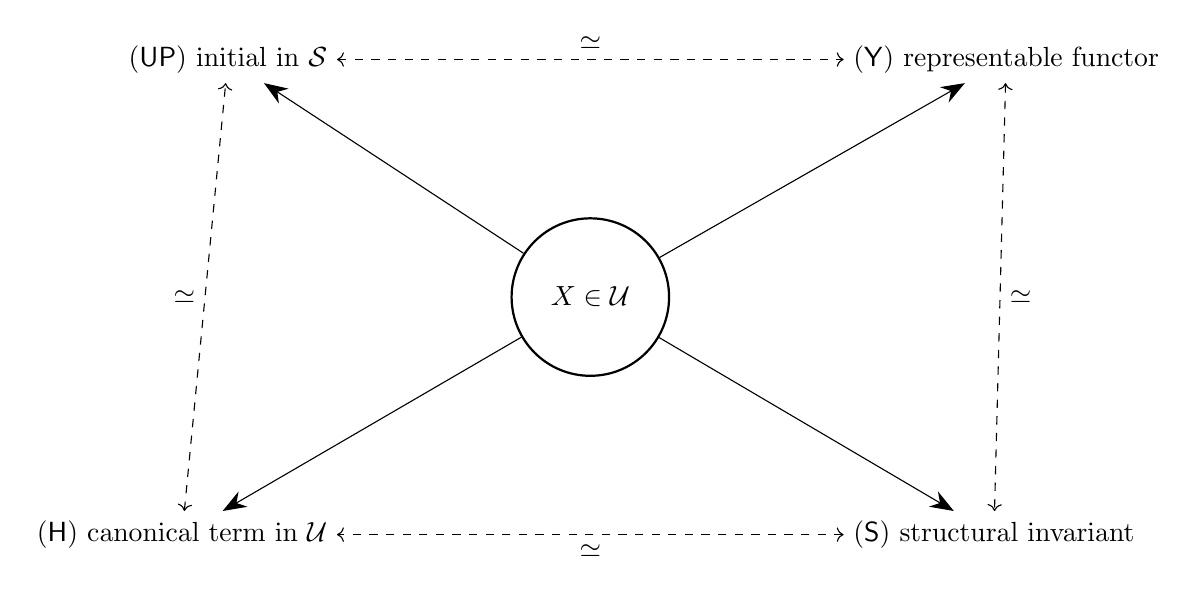
\begin{tikzpicture}[node distance=2.0cm and 2.5cm]
\node (X) [draw, circle, minimum size=2cm, thick] {$X \in \U$};
\node (UP) [above left=of X] {$(\mathsf{UP})$ initial in $\mathcal{S}$};
\node (Y) [above right=of X] {$(\mathsf{Y})$ representable functor};
\node (H) [below left=of X] {$(\mathsf{H})$ canonical term in $\U$};
\node (S) [below right=of X] {$(\mathsf{S})$ structural invariant};
\draw[-{Stealth[length=3mm]}] (X) -- (UP);
\draw[-{Stealth[length=3mm]}] (X) -- (Y);
\draw[-{Stealth[length=3mm]}] (X) -- (H);
\draw[-{Stealth[length=3mm]}] (X) -- (S);
\draw[<->, dashed] (UP) -- (Y) node[midway, above] {$\eqv$};
\draw[<->, dashed] (Y) -- (S) node[midway, right] {$\eqv$};
\draw[<->, dashed] (S) -- (H) node[midway, below] {$\eqv$};
\draw[<->, dashed] (H) -- (UP) node[midway, left] {$\eqv$};
\end{tikzpicture}
\caption{One $\infty$-groupoid, four windows. The four functors of
\cref{def:four-functors} produce the four characterisations of $X$. Under
univalence and SIP, all four characterisations are pairwise equivalent
(\cref{thm:identity-of-perspectives}).}
\label{fig:four-views}
\end{figure}

\subsection{Stratification by homotopy level}

The $\infty$-groupoid view stratifies. For the natural number type $\N$,
which is a $0$-type (a set, in the HoTT Book's $n$-type indexing where
contractible types are $(-2)$-types) by~\cite[Theorem~7.1.6]{HoTTBook}, the
$\infty$-groupoid of NNOs is in fact a contractible $\infty$-groupoid, by
\cref{thm:nno-contr}. So the path space between any two NNO presentations
is itself contractible: the canonical iso between $\N_v$ and $\N_z$ is
not just unique up to ambient choices but \emph{essentially uniquely
unique}, with all higher coherences automatic. This is what
\cref{thm:nno-contr} achieves that mere Peano-equivalence does not.

For $\R$, defined as a higher inductive--inductive type via Cauchy
completion~\cite{Booij,HoTTBook}, the situation is more delicate: $\R$ is
a set ($0$-type) under the propositional truncation conditions of the
HIIT, but the construction of $\R$ from $\Q$ involves higher path
constructors. The transcendentals $\pi$ and $e$ then appear as definite
(canonical-up-to-path) inhabitants of $\R$ via universal-property
characterisations
($\sin(\pi) = 0$, $f' = f$ and $f(0) = 1$, etc.); see \cref{sec:applications}.

\section{The Univalent Correspondence: Statement and Consequences}
\label{sec:correspondence}

We now state the principle systematically.

\begin{principle}[The univalent correspondence, formal version]
\label{prin:formal}
Let $\mathcal{S}$ be a notion of structure given by an essentially
algebraic theory in HoTT. Let $X, Y$ be $\mathcal{S}$-structures in a
univalent universe $\U$. Then the following are pairwise equivalent in
$\U$:
\begin{itemize}
\item[\textsc{(I)}] $X$ and $Y$ both have the same universal property
(both initial, both terminal, both representing the same functor, etc.).
\item[\textsc{(II)}] The Yoneda embeddings $h_X$ and $h_Y$ are
isomorphic as presheaves.
\item[\textsc{(III)}] $\mathsf{H}(X) =_\U \mathsf{H}(Y)$ as types
(identity in the universe).
\item[\textsc{(IV)}] $X$ and $Y$ are equal as elements of the type of
$\mathcal{S}$-structures.
\end{itemize}
The equivalences \textsc{(I)}~$\Leftrightarrow$~\textsc{(II)} and
\textsc{(II)}~$\Leftrightarrow$~\textsc{(III)} are theorems; the
equivalence \textsc{(III)}~$\Leftrightarrow$~\textsc{(IV)} requires the
structure identity principle (a theorem in HoTT, established for
finite-signature structures in~\cite{HoTTBook,Escardo2019}). The
equivalence \textsc{(I)}~$\Leftrightarrow$~\textsc{(IV)} requires
univalence.
\end{principle}

\subsection{The fixed-point reading}

\Cref{prin:formal} can be read as a fixed-point statement. The four
columns of the computational tetrad (\cref{tab:tetrad}) describe four
languages for talking about objects: logic, type theory, category
theory, homotopy theory. Univalence is the assertion that, for the
universe of types, the four languages have a common semantic
fixed point: a single $\infty$-groupoid that satisfies all four
descriptions simultaneously, with the four descriptions identified along
the chain of equivalences just listed.

\begin{remark}[Curry--Howard--Lambek--Voevodsky]
The Curry--Howard correspondence~\cite{Wadler2015} identifies columns~1
and~2 (logic with type theory). The Curry--Howard--Lambek
correspondence~\cite{Lambek1972,maclane} adds column~3 (category theory).
Voevodsky's univalent foundations~\cite{Voevodsky,HoTTBook} adds
column~4 (homotopy theory) by interpreting types as $\infty$-groupoids
and asserting univalence. The univalent correspondence is the strong
form of the four-way Curry--Howard--Lambek--Voevodsky correspondence.
\end{remark}

\subsection{Application to the natural numbers}

\begin{corollary}[The natural numbers are univalent]
\label{cor:N-univalent}
Let $\NNO$ be the type of NNO structures in $\U$. The following are all
the same data, up to canonical equivalence:
\begin{itemize}
\item the universal-property data $(N, 0, \suc, \mathsf{isInitial})$;
\item the representable presheaf $h_N \in [\NNO\op, \U]$;
\item the canonical inhabitant of the contractible type $\NNO$;
\item the iso-class $[(N, 0, \suc)]$ in $\NNO/\eqv$.
\end{itemize}
The integer $58$, defined as $\suc^{58}\,\zero$, is invariant under all
four identifications.
\end{corollary}

\begin{proof}
Combine \cref{thm:nno-contr,thm:identity-of-perspectives,thm:transit-vi}.
\end{proof}

\subsection{Why this resolves the original question}

The original question of the series, ``what is $58$?'', has now four
equivalent answers, each made precise by one of Papers~III through~VI:
\begin{itemize}
\item \emph{(III)} $58$ is the unique element such that, for every pointed
endo-system $(X, x_0, f)$ in any category with terminal object, the unique
NNO morphism $h\colon \N \to X$ sends $58$ to $f^{58}(x_0)$.
\item \emph{(IV)} $58$ is the natural number whose representable functor
$\Hom(-, 58)$, under the Yoneda embedding into the presheaf topos, exhibits
all probes onto $58$ from below.
\item \emph{(V)} $58$ is the canonical term $\suc^{58}\,\zero : \N$,
identified with $\suc^{58}\,\zero$ in any equivalent NNO presentation by
transport along the unique path in the contractible type $\NNO$.
\item \emph{(VI)} $58$ is the value of any (every) definable arithmetic
quantity that, on the standard model of arithmetic, evaluates to $58$;
this value is invariant under all model isomorphisms by SIP.
\end{itemize}
The univalent correspondence asserts that these four answers are not just
\emph{about} the same object: they are \emph{the same data}, internally,
in HoTT.

\section{Hierarchical Composition: How Each Level Builds on the Previous}
\label{sec:diagrams}

The univalent correspondence is not just a parallel array of four
descriptions: it is a hierarchical composition in which each level uses
the data of the previous one. We make the dependencies explicit.

\subsection{Composition diagram}

\Cref{fig:composition} shows the dependencies between the six rows.

\begin{figure}[ht]
\centering
\begin{tikzcd}[
  column sep={2.0em,between origins},
  row sep=2.4em,
  every label/.append style={font=\scriptsize}
]
\text{(I) Naive}
  \arrow[r, "{\text{T1}}"]
& \text{(II) Set-th.}
  \arrow[r, "{\text{T2}}"]
& \text{(III) U.P.}
  \arrow[r, "{\text{T3}}"]
& \text{(IV) Yoneda}
  \arrow[r, "{\text{T4}}"]
& \text{(V) HoTT}
  \arrow[r, "{\text{T5}}"]
& \text{(VI) Struct.}
\end{tikzcd}
\caption{Hierarchical composition: each transit theorem T$k$ of
\cref{sec:transit} carries level $k$ to level $k+1$ by resolving the
residual question of the previous level. T1 supplies a definite encoding
(resolving the symbol/object confusion). T2 abstracts away from the
Benacerraf-non-canonical encoding. T3 globalises the universal property
by exhibiting the NNO as a representable functor. T4 internalises
Yoneda's ``iff'' as a path in the universe via univalence. T5
(\cref{thm:transit-vi}) promotes the iso-invariance discipline to an
internal theorem via SIP.}
\label{fig:composition}
\end{figure}

\subsection{Composition is not optional}

A natural objection: if all four formal levels (III--VI) are equivalent
under univalence, why bother with all four? Why not just use HoTT?

The answer is that each level supplies indispensable conceptual content
that the others alone would obscure:
\begin{itemize}
\item The universal property (III) is what \emph{lets us recognise} an
NNO when we see one. We do not begin in HoTT and then notice that the
inductive type $\N$ is initial; we begin with the universal property as
a design constraint and use it to determine what the type-theoretic data
must look like.
\item Yoneda (IV) is the bridge that lets us speak of the universal
property \emph{relationally}, in any background category, not just inside
HoTT. The Yoneda embedding is what we use when working with categories
of geometric or algebraic objects (schemes, groups, manifolds) where the
HoTT presentation is not yet fully developed.
\item HoTT (V) is what \emph{internalises} the equivalence: it is the
formal system in which ``up to iso'' becomes ``equal.''
\item The categorical / structural perspective (VI) is the philosophical
commitment that drives the whole programme. Without it, we have no
reason to prefer one perspective over another; with it, we know what
we are doing.
\end{itemize}

\subsection{Emergent properties from composition}

The hierarchical composition produces emergent properties not visible at
any single level. We collect three.

\begin{proposition}[Emergent property: contractibility of NNO]
\label{prop:emergent-contract}
The NNO is contractible (Paper~V, \cref{thm:nno-contr}) only because the
universal property (III) gives a unique map between any two NNOs, the
Yoneda embedding (IV) gives that this unique map is an isomorphism, and
the univalence axiom (V) promotes the isomorphism to a path. Set theory
(II) alone gives only that the von Neumann and Zermelo encodings are
isomorphic as Peano structures: the structure-of-paths between them is not
visible at the set-theoretic level.
\end{proposition}

\begin{proposition}[Emergent property: function extensionality]
\label{prop:funext}
Function extensionality is provable from univalence
(\cite[\S4.9]{HoTTBook}, see Paper~V \S4). It is not provable
from intensional Martin-L\"of type theory alone, nor from the universal
property of any individual structure. It emerges from the composition of
universal property, Yoneda, and univalence.
\end{proposition}

\begin{proposition}[Emergent property: synthetic homotopy theory]
\label{prop:synth-homotopy}
Synthetic homotopy theory (the development of algebraic topology entirely
inside type theory: $\pi_1(S^1) \iso \Z$, the Hopf fibration, the
Blakers--Massey theorem, etc.~\cite{LicataShulman,LicataFinster,ShulmanStrength})
is impossible at any of the levels (I), (II), (III), or (IV) alone. It
emerges from the composition: the categorical perspective (VI) supplies
the $\infty$-groupoid view, HoTT (V) gives identity types as path spaces,
the Yoneda principle (IV) recovers presentability, and the universal
property (III) gives recursion principles for the higher inductive types.
\end{proposition}

\subsection{Commutativity of the four-functor diagram}

\begin{theorem}[Commutativity]
\label{thm:commutativity}
The four functors of \cref{def:four-functors} commute up to canonical
natural equivalence: for every $X \in \U$,
\[
\mathsf{S} \circ \mathsf{H}^{-1} \circ \mathsf{Y}\,(X) \,\eqv\, \mathsf{UP}(X)
\]
in the appropriate sense, where the inverses are well-defined modulo
contractibility of fibers (which holds for finite-signature structures by
SIP).
\end{theorem}

\begin{proof}[Sketch]
Each pair is treated by the corresponding transit theorem of
\cref{sec:transit}. The composition $\mathsf{S} \circ \mathsf{H}^{-1} \circ \mathsf{Y}$
takes a structure to its representable presheaf, transports back to a
type-theoretic representative, and projects to its iso-class; this is the
same data as the universal-property witness for $X$, after suppressing the
choice of representative. Naturality follows from the naturality of each
constituent.
\end{proof}

\section{Naming the Correspondence: A Brief History}
\label{sec:naming}

We pause to justify our terminology. The four-way correspondence has many
names; we explain why we settle on \emph{the univalent correspondence}.

\subsection{Names in use}

\begin{itemize}
\item \textbf{Curry--Howard correspondence} (binary): logic with type
theory. Curry (1934)~\cite{wadler-pat} observed it for combinatory logic;
Howard (1969)~\cite{wadler-pat} extended it to natural deduction.
\item \textbf{Curry--Howard--Lambek} (three-way): adds category theory.
Lambek (1972)~\cite{Lambek1972} showed that proofs of intuitionistic
propositional logic and typed combinators share the equational theory of
cartesian closed categories; this is the textbook three-way name.
\item \textbf{Computational trinity} (Harper, c.\ 2011): logic, languages
(type theory), categories. Harper at CMU popularised the catchier name. A
four-way version is sometimes called the computational tetrad.
\item \textbf{Propositions-as-types} (Wadler 2015~\cite{Wadler2015}):
emphasises the central insight rather than the historical figures.
Extends naturally to ``propositions-as-types-as-spaces'' in HoTT.
\item \textbf{Univalent foundations} (Voevodsky, 2010~\cite{Voevodsky2010}):
the foundational programme built on the four-way correspondence. Homotopy
Type Theory (HoTT) is the formal system; the
HoTT Book~\cite{HoTTBook} is the canonical reference.
\end{itemize}

\subsection{Why ``the univalent correspondence''}

The phrase ``Curry--Howard--Lambek--Voevodsky correspondence'' is correct
but unwieldy. ``Propositions as types as spaces'' is pedagogically apt
but emphasises types and propositions over the unifying mechanism. We
prefer \emph{the univalent correspondence} for three reasons:
\begin{enumerate}
\item It \emph{names the unifying mechanism}: the univalence axiom is
what promotes the four columns from analogous to literally the same.
\item It is \emph{neutral across the columns}: it does not privilege
logic, types, categories, or spaces.
\item It \emph{credits the discovery}: Voevodsky's univalent foundations
project is the conceptual origin of the strong form
(\cref{prin:strong}).
\end{enumerate}

We also use \emph{the $\infty$-groupoid correspondence} when emphasising
the underlying object, and \emph{structural univalence} when emphasising
the philosophical commitment of Paper~VI.

\subsection{The deepest formulation}

For the record, the most precise summary of the unified language is the
one from~\cite{Voevodsky2010,HoTTBook}, which we take as the deepest
formulation of the univalent correspondence:

\begin{quote}
The unified language is \emph{synthetic homotopy theory} expressed as
\emph{dependent type theory}, with categorical semantics in
\emph{$(\infty,1)$-toposes}, interpreted logically via
\emph{propositions-as-types}. The whole package is
\emph{Univalent Foundations}.
\end{quote}

\section{Applications and Outlook}
\label{sec:applications}

We close with three applications that the univalent correspondence
illuminates.

\subsection{Transcendentals \texorpdfstring{$\pi$ and $e$}{pi and e} in HoTT}
\label{sec:transcendentals}

The transcendental numbers $\pi$ and $e$ enter the framework via Paper~V's
HIIT real numbers and Paper~III's universal-property characterisations.

\begin{definition}[Cauchy real numbers, HIIT, Paper~V \S5.5]
\label{def:R-HIIT}
The type $\R_C$ of Cauchy real numbers is the higher inductive--inductive
type freely generated by:
\begin{itemize}
\item $\mathsf{rat}\colon \Q \to \R_C$;
\item $\mathsf{lim}\colon \prod_{f : \N \to \R_C}\, \mathsf{isCauchy}(f) \to \R_C$;
\item path constructors identifying $\mathsf{lim}\,f$ for any two
representations of the same Cauchy class;
\item the truncation that makes $\R_C$ a set.
\end{itemize}
\end{definition}

\begin{theorem}[$\pi$ and $e$ in HoTT, after Paper~V \S10]
\label{thm:pi-e-hott}
There exist canonical inhabitants $\pi, e : \R_C$ characterised by the
unique-existence propositions:
\begin{itemize}
\item $\pi$ is the unique inhabitant of the truncated $\Sigma$-type
$\sum_{x : \R_C} (x > 0) \times (\sin x = 0) \times (\forall y \in (0, x).\, \sin y > 0)$;
\item $e$ is the unique inhabitant of the truncated $\Sigma$-type
$\sum_{x : \R_C} (\exp x = e) \times (\exp 0 = 1) \times (\exp' = \exp)$,
where $\exp$ is defined by power series.
\end{itemize}
The truncation makes the $\Sigma$-types mere propositions ($(-1)$-types),
hence inhabitants are unique up to a unique path.
\end{theorem}

The univalent correspondence applies to $\pi$ and $e$ as it does to $58$:
each is identified with its representable functor, with its universal
property (\emph{half-period of} $\exp\colon \R \to S^1$, \emph{unique fixed
point of differentiation with} $f(0) = 1$), with its structural invariant
under field automorphisms of $\R$, and with its canonical HoTT term up to
path equivalence.

\subsection{ContextFS as a structural-identity primitive}
\label{sec:contextfs}

The ContextFS / typed memory project~\cite{KnowledgeBase2026} aims to
provide AI agents with persistent typed memory that respects structural
identity. The univalent correspondence supplies the theoretical foundation:
two memory entries should be considered ``the same'' iff they witness the
same structural invariant, iff they correspond to equal types in the
ambient universe, iff they have the same Yoneda profile in the category
of memory operations, iff they satisfy the same universal property.

We sketch the architecture. A typed memory is a presheaf
$M\colon \mathsf{Op}\op \to \U$ on the category of memory operations, where
$\U$ is a univalent universe of types. The universal-property layer
specifies which operations any memory entry must support; the Yoneda
layer makes ``same memory entry'' precise as natural isomorphism of
presheaves; the HoTT layer makes ``natural isomorphism'' a path in $\U$;
the categorical/structural layer ensures that all of this is preserved
under change of universe (e.g.\ when the agent is migrated).

\begin{principle}[ContextFS univalent slogan]
A memory entry is identified by its structural role, not by its storage
location.
\end{principle}

This is precisely the univalent correspondence applied to a different
domain: instead of $58$, the entry is identified by what it does, not by
where it lives.

\subsection{Directed HoTT and synthetic \texorpdfstring{$\infty$}{Infinity}-category theory}
\label{sec:directed}

Riehl and Shulman's simplicial type theory~\cite{RiehlShulman} extends
HoTT with directed structure, allowing types whose paths are not
necessarily invertible. This is the language of synthetic
$\infty$-category theory: an $\infty$-category is a type with a chosen
directed structure satisfying the Segal and Rezk conditions internally.

The univalent correspondence applies in the directed setting too, but
modulo a shift: ``equality of objects'' becomes ``isomorphism of objects''
(an invertible path), distinct from ``$X$ maps to $Y$'' (a possibly
non-invertible morphism). This is the right setting for
representation theory, where representations are functors that need not
be equivalences. We sketch the upshot in the language of Paper~VI: a
representation $\rho\colon G \to \mathsf{Vect}$ is a directed map; a
sub-representation is an iso-mono in the directed sense; the
representation theory of finite groups becomes a synthetic theory of
directed types over the classifying type $BG$.

\subsection{Open problem: analytic number theory in HoTT}
\label{sec:open-langlands}

The principal open problem the series acknowledges is that analytic number
theory --- Riemann zeta zeros, the Langlands programme, automorphic
forms~\cite{lurie} --- has not been substantially reformulated in HoTT.
Algebraic number theory and parts of arithmetic geometry (schemes, sheaves,
\'etale cohomology) admit $(\infty,1)$-topos and condensed mathematics
treatments~\cite{ShulmanInftyTopos} that connect cleanly to univalent
foundations. But $\zeta(s) = 0$ as a HoTT-native statement, with $\zeta$ a
HoTT-native object, remains unrealised.

We frame this as the principal open question for the synthesis.

\section{Open Problems}
\label{sec:open}

We collect the open problems flagged by the topical papers and by the
synthesis.

\begin{enumerate}
\item \textbf{Coalgebraic / final-object dual for transcendentals.}
Paper~III sketches the coalgebraic side: streams of digits, codata,
bisimulation as the corresponding induction principle. A complete
final-coalgebra characterisation of $\pi$ and $e$ that avoids the
inductive HIIT route is open.
\item \textbf{Connections to Langlands and analytic number theory.}
\Cref{sec:open-langlands}.
\item \textbf{ETCS, IZF, and FOLDS as alternative structural foundations.}
Paper~VI surveys ETCS; the relationship to Makkai's
FOLDS~\cite{Makkai1995} and to intuitionistic ZF (IZF) merits
development.
\item \textbf{Higher-categorical structure of NNO.} The contractibility
result (\cref{thm:nno-contr}) shows the type of NNOs is a contractible
type (a $(-2)$-type). The corresponding statement for $(\infty,1)$-NNOs in
$\infty$-toposes (Lurie's $(\infty,1)$-NNO~\cite{lurie}) is more delicate.
\item \textbf{ContextFS / type-memory as a structural-identity primitive.}
A formal account of typed persistent memory in HoTT, with structural
identity as the primitive notion, is the principal applied research
direction.
\item \textbf{Directed univalence.} Riehl and Shulman's simplicial type
theory has a partial directed univalence; a complete principle remains a
research target~\cite{RiehlShulman,CisinskiNguyen}.
\item \textbf{Cubical higher inductive--inductive types.} The Cauchy
reals construction of Paper~V is given in Book HoTT; a clean cubical
version (in Cubical Agda~\cite{CubicalAgda}) is in progress but
incomplete.
\end{enumerate}

\section{Conclusion}
\label{sec:conclusion}

We have argued that the question \emph{what is the natural number $58$?}
admits six progressively refined answers, and that the four most refined
answers are not analogous but \emph{literally the same} under Voevodsky's
univalence axiom. We named this identification the \emph{univalent
correspondence} (\cref{prin:strong}, \cref{prin:formal}), proved it as a
theorem in HoTT (\cref{thm:identity-of-perspectives}), exhibited the
hierarchical composition by which each level builds on the previous
(\cref{sec:diagrams}), and sketched applications to transcendentals,
typed memory, and directed type theory.

The integer $58$ is, in the unified picture: a position in the initial
successor structure (Paper~III), a representing functor (Paper~IV), a
canonical term in a contractible type of NNOs (Paper~V), and an
invariant under all model isomorphisms (Paper~VI). These four
characterisations are four windows on a single $\infty$-groupoid, and
under univalence they are pairwise identified. The univalent correspondence
is the formal expression of the structuralist intuition that mathematical
objects are positions in structures, not substances; under Voevodsky's
univalent foundations, this intuition becomes a theorem of the
foundations themselves.

The naive level (Paper~I), in which $58$ is a symbol on a page, remains
indispensable as the cognitive anchor that connects mathematics to human
practice. The set-theoretic level (Paper~II) remains the historical and
technical foundation for working mathematicians, and the von Neumann
encoding remains the textbook construction. But the univalent
correspondence asserts that these levels are not the locus of meaning:
the meaning lives at levels III through VI, where it is invariant,
relational, type-theoretic, and structural --- and, under univalence, all
four at once.

We close with the canonical quotation that has guided the series, from
Paper~I:

\begin{quote}
A number is not a thing. It is a constraint that every consistent
representation must satisfy, identified by a universal property and made
formal by its representable functor. Numerals (58, \textsf{LVIII},
$\,||||\,||||$) are syntax. Numbers are semantic invariants of the
categories that admit them.
\end{quote}

\noindent The univalent correspondence makes this slogan a theorem.

\section{The Haskell Artifact}
\label{sec:haskell}

The companion repository ships a small Haskell program that demonstrates
the synthesis claim computationally: six executable witnesses that all
return the same number when asked ``what is $58$?'' The program lives in
\verb|src/07-synthesis/| and consists of three modules.

\paragraph{\normalfont\texttt{Synthesis.hs}.} Defines a six-element
enumeration
\begin{lstlisting}[language=Haskell]
data Perspective
  = Naive | SetTheoretic | UniversalProperty
  | Yoneda | HoTT | StructuralInvariant
\end{lstlisting}
together with the trivially uniform map
\verb|answer :: Perspective -> Int -> Int|. The point is precisely that
\verb|answer p n = n| for every perspective \verb|p|: the perspective is
discharged by transport.

\paragraph{\normalfont\texttt{UnifiedNumber.hs}.} Implements one numerical witness
per row of \cref{tab:six-rows}:
\begin{itemize}
\item \emph{Naive:} the literal \verb|58|.
\item \emph{Set-theoretic:} \verb|vonNeumannCard 58|, returning the
cardinality of the von Neumann encoding.
\item \emph{Universal property:} \verb|toIntL (succIterate 58 :: Peano)|,
applying the unique map out of the NNO into the Peano model.
\item \emph{Yoneda:} \verb|predecessorsOf 58|, the cardinality of
$\{m : \mathrm{Hom}(m, 58) \neq \emptyset\}$ in the order category, by
the Yoneda lemma equal to $58$.
\item \emph{HoTT:} the length of the canonical successor chain
$\zero \mapsto \mathsf{succ}\,\zero \mapsto \cdots \mapsto 58$ in
$\N$, identified up to path equivalence.
\item \emph{Structural:} \verb|finiteOrbitLength 59 1|, the number of
successor steps required to send $1$ back to $0$ in the cyclic carrier
$\mathbb{Z}/59\mathbb{Z}$ under $s(x) = x + 1 \bmod 59$. This count is
$58$, and by \cref{thm:transit-vi} it is invariant across all isomorphic
presentations of the carrier.
\end{itemize}

\paragraph{\normalfont\texttt{Main.hs}.} Runs all six computations and verifies that
they all agree on $58$. The recorded transcript is:
\begin{lstlisting}[language={}]
The Univalent Correspondence -- six perspectives, one answer
=============================================================

Perspective-tagged answer for n = 58:
  Naive                  -> 58
  SetTheoretic           -> 58
  UniversalProperty      -> 58
  Yoneda                 -> 58
  HoTT                   -> 58
  StructuralInvariant    -> 58

Unified computation across the six rows of the columns table:
  naive                              = 58
  set-theoretic (von Neumann)        = 58
  universal property (succ^58)       = 58
  Yoneda (|{m : Hom(m,58) /= 0}|)    = 58
  HoTT (|0 =_N 58 chain|)            = 58
  structural (orbit length)          = 58

All six perspectives agree on 58? True
\end{lstlisting}

The program compiles clean under \verb|-Wall -Wextra -Werror| and runs
to completion. It is not a proof of the synthesis claim, only a
finite executable witness consistent with it; the proofs are inside
Papers~I--VI and \S\ref{sec:transit}.

\section*{Acknowledgments}

This synthesis owes its existence to the topical papers~I through~VI, to
the body of work surveyed in those papers (Lawvere, Mac Lane, Lambek,
Martin-L\"of, Voevodsky, Awodey, Shulman, Riehl, Lurie, Wadler, Harper,
the Univalent Foundations Programme), and to the philosophical lineage of
Frege, Benacerraf, Resnik, Shapiro, and Hellman. The naming
``univalent correspondence'' is internal to this project and is not
claimed to be original; the underlying mathematical content is due to the
named authors.

\begin{thebibliography}{99}

% --- Topical papers in this series ---

\bibitem{paper-i}
YonedaAI Research,
\emph{The Naive Perspective: Numbers as Symbols and Quantities},
Univalent Correspondence Series, Paper~I, 2026.

\bibitem{paper-ii}
YonedaAI Research,
\emph{The Set-Theoretic Perspective: Numbers as von Neumann Ordinals},
Univalent Correspondence Series, Paper~II, 2026.

\bibitem{paper-iii}
YonedaAI Research,
\emph{The Universal Property Perspective: Numbers as Initial Successor Structures},
Univalent Correspondence Series, Paper~III, 2026.

\bibitem{paper-iv}
YonedaAI Research,
\emph{The Yoneda Perspective: Numbers as Representable Functors},
Univalent Correspondence Series, Paper~IV, 2026.

\bibitem{paper-v}
YonedaAI Research,
\emph{The HoTT Perspective: Numbers as Inductive Types up to Path Equivalence},
Univalent Correspondence Series, Paper~V, 2026.

\bibitem{paper-vi}
YonedaAI Research,
\emph{The Categorical / Structural Perspective: Numbers as Invariants of Structure-Preserving Morphisms},
Univalent Correspondence Series, Paper~VI, 2026.

\bibitem{KnowledgeBase2026}
YonedaAI Research,
\emph{Knowledge Base: The Univalent Correspondence},
Magneton Internal Document, 2026.

% --- Foundations of HoTT and univalence ---

\bibitem{HoTTBook}
The Univalent Foundations Program,
\emph{Homotopy Type Theory: Univalent Foundations of Mathematics},
Institute for Advanced Study, 2013.
\texttt{arXiv:1308.0729}.

\bibitem{Voevodsky}
V.~Voevodsky,
\emph{The equivalence axiom and univalent models of type theory},
\texttt{arXiv:1402.5556}, 2014.

\bibitem{Voevodsky2010}
V.~Voevodsky,
\emph{Univalent foundations project},
Manuscript, IAS, 2010.

\bibitem{AwodeyWarren}
S.~Awodey and M.~A.~Warren,
\emph{Homotopy theoretic models of identity types},
Math.\ Proc.\ Cambridge Philos.\ Soc.\ \textbf{146}(1): 45--55, 2009.

\bibitem{KapulkinLumsdaine}
C.~Kapulkin and P.~L.~Lumsdaine,
\emph{The simplicial model of univalent foundations (after Voevodsky)},
J.\ Eur.\ Math.\ Soc.\ \textbf{23}(6): 2071--2126, 2021.

\bibitem{LumsdaineGroupoid}
P.~L.~Lumsdaine,
\emph{Weak omega-categories from intensional type theory},
Logical Methods in Computer Science \textbf{6}(3:24): 1--19, 2010.

\bibitem{vandenBergGarner}
B.~van den Berg and R.~Garner,
\emph{Types are weak omega-groupoids},
Proc.\ London Math.\ Soc.\ \textbf{102}(2): 370--394, 2011.

\bibitem{LicataShulman}
D.~R.~Licata and M.~Shulman,
\emph{Calculating the fundamental group of the circle in homotopy type theory},
in LICS 2013, pp.~223--232.

\bibitem{LicataFinster}
D.~R.~Licata and E.~Finster,
\emph{Eilenberg--MacLane spaces in homotopy type theory},
in CSL-LICS 2014, ACM, 2014.

\bibitem{ShulmanStrength}
M.~Shulman,
\emph{Higher inductive types and the formal Blakers--Massey theorem},
Proc.\ ACM Program.\ Lang.\ \textbf{4}(POPL): 41:1--41:30, 2020.

\bibitem{ShulmanInftyTopos}
M.~Shulman,
\emph{All $(\infty,1)$-toposes have strict univalent universes},
\texttt{arXiv:1904.07004}, 2019.

\bibitem{Booij}
A.~B.~Booij,
\emph{Analysis in univalent type theory},
PhD thesis, University of Birmingham, 2020.

\bibitem{CCHM}
C.~Cohen, T.~Coquand, S.~Huber, A.~M\"ortberg,
\emph{Cubical type theory: a constructive interpretation of the univalence axiom},
in TYPES 2015, LIPIcs 69, pp.~5:1--5:34.

\bibitem{CubicalAgda}
A.~Vezzosi, A.~M\"ortberg, A.~Abel,
\emph{Cubical Agda: a dependently typed programming language with univalence and higher inductive types},
Proc.\ ACM Program.\ Lang.\ \textbf{3}(ICFP): 87:1--87:29, 2019.

\bibitem{2LTT}
D.~Annenkov, P.~Capriotti, N.~Kraus, C.~Sattler,
\emph{Two-level type theory and applications},
Math.\ Structures Comput.\ Sci.\ \textbf{33}(8): 688--743, 2023.

\bibitem{RiehlShulman}
E.~Riehl and M.~Shulman,
\emph{A type theory for synthetic $\infty$-categories},
Higher Structures \textbf{1}(1): 147--224, 2017.
\texttt{arXiv:1705.07442}.

\bibitem{CisinskiNguyen}
D.-C.~Cisinski and H.~K.~Nguyen,
\emph{The universal coCartesian fibration},
\texttt{arXiv:2210.08945}, 2022.

\bibitem{Escardo2019}
M.~H.~Escard\'o,
\emph{Introduction to Univalent Foundations of Mathematics with Agda},
Lecture notes, 2019.

% --- Type theory and Curry--Howard ---

\bibitem{MartinLof84}
P.~Martin-L\"of,
\emph{Intuitionistic Type Theory},
Bibliopolis, 1984.

\bibitem{Wadler2015}
P.~Wadler,
\emph{Propositions as types},
Communications of the ACM \textbf{58}(12): 75--84, 2015.

\bibitem{Lambek1972}
J.~Lambek,
\emph{Deductive systems and categories III: Cartesian closed categories,
intuitionist propositional calculus, and combinatory logic},
in Toposes, Algebraic Geometry and Logic, LNM 274, Springer, 1972, 57--82.

% --- Category theory ---

\bibitem{maclane}
S.~Mac Lane,
\emph{Categories for the Working Mathematician},
2nd ed., Graduate Texts in Mathematics \textbf{5}, Springer, 1998.

\bibitem{maclane-moerdijk}
S.~Mac Lane and I.~Moerdijk,
\emph{Sheaves in Geometry and Logic: A First Introduction to Topos Theory},
Springer, 1992.

\bibitem{riehl}
E.~Riehl,
\emph{Category Theory in Context},
Aurora: Dover Modern Math Originals, Dover, 2016.

\bibitem{lurie}
J.~Lurie,
\emph{Higher Topos Theory},
Annals of Mathematics Studies \textbf{170}, Princeton, 2009.
\texttt{arXiv:math/0608040}.

\bibitem{kelly}
G.~M.~Kelly,
\emph{Basic Concepts of Enriched Category Theory},
LMS Lecture Note Series \textbf{64}, Cambridge University Press, 1982.

\bibitem{leinster}
T.~Leinster,
\emph{Basic Category Theory},
Cambridge Studies in Advanced Mathematics \textbf{143}, Cambridge University Press, 2014.

\bibitem{Lawvere1964}
F.~W.~Lawvere,
\emph{An elementary theory of the category of sets},
Proc.\ Nat.\ Acad.\ Sci.\ USA \textbf{52}(6): 1506--1511, 1964.

\bibitem{Lawvere1963}
F.~W.~Lawvere,
\emph{Functorial semantics of algebraic theories},
PhD thesis, Columbia University, 1963.

\bibitem{LawvereRosebrugh2003}
F.~W.~Lawvere and R.~Rosebrugh,
\emph{Sets for Mathematics},
Cambridge University Press, 2003.

\bibitem{Makkai1995}
M.~Makkai,
\emph{First-order logic with dependent sorts, with applications to category theory},
Preprint, McGill University, 1995.
\url{https://www.math.mcgill.ca/makkai/folds/foldsinpdf/FOLDS.pdf}

\bibitem{MeijerFokkingaPaterson1991}
E.~Meijer, M.~Fokkinga, and R.~Paterson,
\emph{Functional programming with bananas, lenses, envelopes, and barbed wire},
in FPCA '91, LNCS 523, Springer, 1991, 124--144.

\bibitem{BaezDolan1998}
J.~C.~Baez and J.~Dolan,
\emph{From finite sets to Feynman diagrams},
in Mathematics Unlimited --- 2001 and Beyond, Springer, 29--50, 2001.

\bibitem{Leinster2008}
T.~Leinster,
\emph{The Euler characteristic of a category},
Documenta Mathematica \textbf{13}: 21--49, 2008.

% --- Set theory ---

\bibitem{vonNeumann1923}
J.~von Neumann,
\emph{Zur Einf\"uhrung der transfiniten Zahlen},
Acta Litt.\ Sci.\ Reg.\ Univ.\ Hung.\ Francisco-Josephinae \textbf{1}: 199--208, 1923.

\bibitem{zermelo1908}
E.~Zermelo,
\emph{Untersuchungen \"uber die Grundlagen der Mengenlehre I},
Math.\ Annalen \textbf{65}: 261--281, 1908.

\bibitem{halmos1960}
P.~Halmos,
\emph{Naive Set Theory},
Van Nostrand, 1960.

\bibitem{kunen1980}
K.~Kunen,
\emph{Set Theory: An Introduction to Independence Proofs},
North-Holland, 1980.

\bibitem{shoenfield1967}
J.~R.~Shoenfield,
\emph{Mathematical Logic},
Addison-Wesley, 1967.

\bibitem{suppes1960}
P.~Suppes,
\emph{Axiomatic Set Theory},
Van Nostrand, 1960.

% --- Philosophy of mathematics ---

\bibitem{benacerraf1965}
P.~Benacerraf,
\emph{What numbers could not be},
Philosophical Review \textbf{74}(1): 47--73, 1965.

\bibitem{benacerraf1973}
P.~Benacerraf,
\emph{Mathematical truth},
Journal of Philosophy \textbf{70}(19): 661--679, 1973.

\bibitem{frege1884}
G.~Frege,
\emph{Die Grundlagen der Arithmetik},
Breslau, 1884.

\bibitem{frege1892}
G.~Frege,
\emph{\"Uber Sinn und Bedeutung},
Zeitschrift f\"ur Philosophie und philosophische Kritik \textbf{100}: 25--50, 1892.

\bibitem{husserl1891}
E.~Husserl,
\emph{Philosophie der Arithmetik},
Halle, 1891.

\bibitem{mill1843}
J.~S.~Mill,
\emph{A System of Logic},
London, 1843.

\bibitem{Resnik1981}
M.~D.~Resnik,
\emph{Mathematics as a science of patterns: Ontology and reference},
No\^us \textbf{15}(4): 529--550, 1981.

\bibitem{Resnik1997}
M.~D.~Resnik,
\emph{Mathematics as a Science of Patterns},
Oxford University Press, 1997.

\bibitem{Shapiro1997}
S.~Shapiro,
\emph{Philosophy of Mathematics: Structure and Ontology},
Oxford University Press, 1997.

\bibitem{Hellman1989}
G.~Hellman,
\emph{Mathematics Without Numbers: Towards a Modal-Structural Interpretation},
Oxford University Press, 1989.

\bibitem{Awodey1996}
S.~Awodey,
\emph{Structure in mathematics and logic: A categorical perspective},
Philosophia Mathematica \textbf{4}(3): 209--237, 1996.

\bibitem{Awodey2004}
S.~Awodey,
\emph{An answer to Hellman's question},
Philosophia Mathematica \textbf{12}(1): 54--64, 2004.

\bibitem{Awodey2014}
S.~Awodey,
\emph{Structuralism, invariance, and univalence},
Philosophia Mathematica \textbf{22}(1): 1--11, 2014.

\bibitem{Dedekind1888}
R.~Dedekind,
\emph{Was sind und was sollen die Zahlen?},
Vieweg \& Sohn, Braunschweig, 1888.

% --- Misc / cognitive science ---

\bibitem{wadler-pat}
P.~Wadler,
\emph{Propositions as types}
(extended discussion of historical names),
CACM \textbf{58}(12): 75--84, 2015.

\bibitem{carey}
S.~Carey,
\emph{The Origin of Concepts},
Oxford University Press, 2009.

\bibitem{dehaene}
S.~Dehaene,
\emph{The Number Sense},
Oxford University Press, 1997.

\bibitem{lakoff-nunez}
G.~Lakoff and R.~N\'u\~nez,
\emph{Where Mathematics Comes From},
Basic Books, 2000.

\end{thebibliography}

\end{document}
